% !TEX root = paper.tex
\section{Experimental Results}\label{sec:results}

\begin{figure}[H]
    \centering
    \begin{subfigure}[t]{0.24\textwidth}
        \centering
        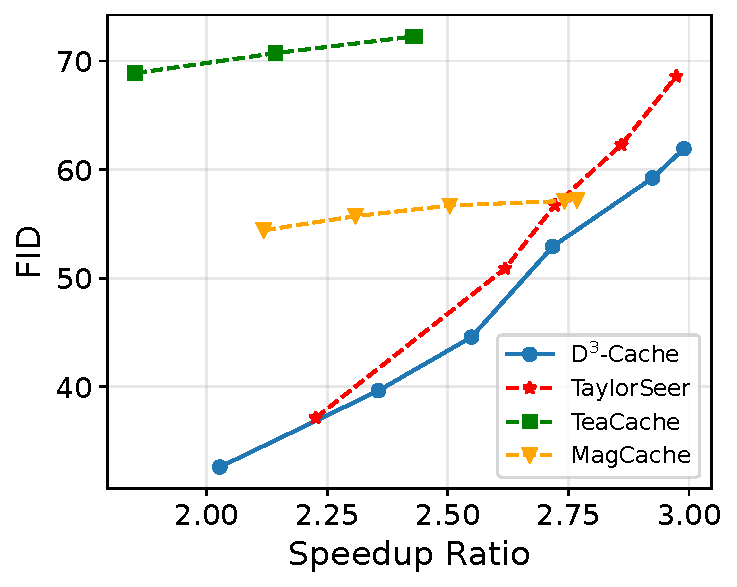
\includegraphics[width=\linewidth, trim=0 0 20pt 0]{figures/results/FID.pdf}
    \end{subfigure}\hfill
    \begin{subfigure}[t]{0.24\textwidth}
        \centering
        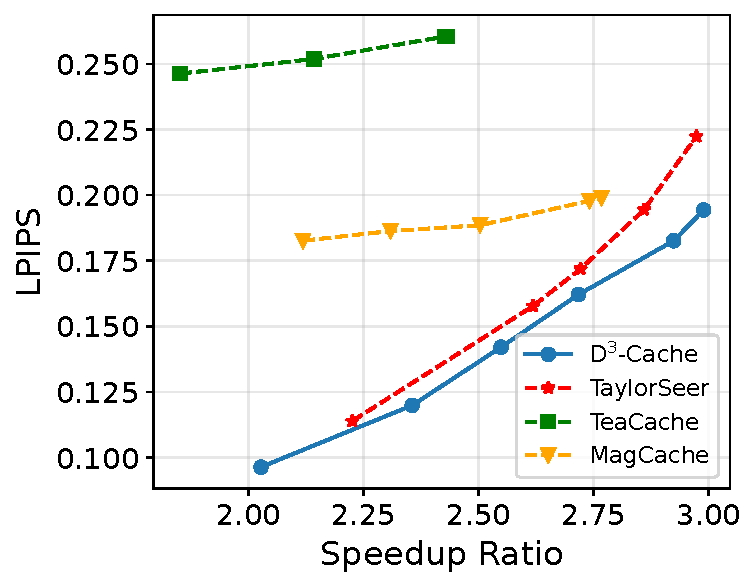
\includegraphics[width=\linewidth, trim=10pt 0 10pt 0]{figures/results/LPIPS.pdf}
    \end{subfigure}\hfill
    \begin{subfigure}[t]{0.24\textwidth}
        \centering
        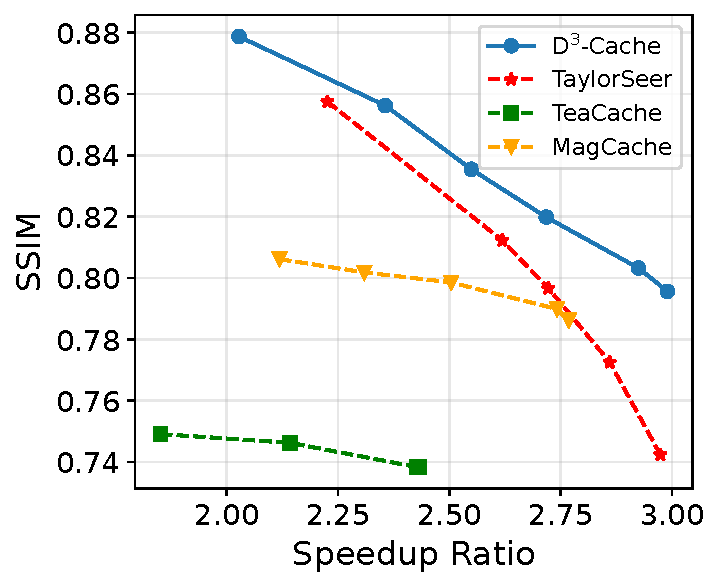
\includegraphics[width=\linewidth, trim=10pt 0 10pt 0]{figures/results/SSIM.pdf}
    \end{subfigure}
    \begin{subfigure}[t]{0.24\textwidth}
        \centering
        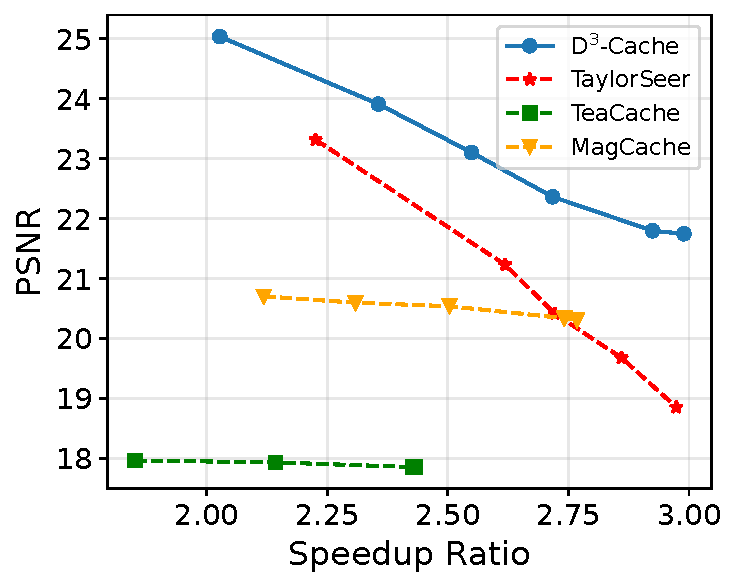
\includegraphics[width=\linewidth, trim=10pt 0 0pt 0]{figures/results/PSNR.pdf}
    \end{subfigure}\hfill
    \caption{
        Quality metrics (FID, LPIPS, PSNR, SSIM) across methods on FLUX.1-dev model.
    }\label{fig:results:metrics}
    \vspace{-10pt}
\end{figure}

\begin{table}[t]
\centering
\begingroup
\setlength{\tabcolsep}{0.25em}
\renewcommand{\arraystretch}{1.08}
\newcolumntype{L}{>{\hspace{0.45em}}l<{\hspace{0.45em}}}
\newcolumntype{C}{>{\hspace{0.35em}}c<{\hspace{0.35em}}}
\begin{tabular}{LCC CCCCC}
\toprule
\multirow{2}{*}{\textbf{Method}}
    & \multicolumn{2}{c}{\textbf{Efficiency}}
    & \multicolumn{5}{c}{\textbf{Visual Quality}} \\
\cmidrule(lr){2-3}\cmidrule(lr){4-8}
    & \textbf{Speedup$\uparrow$}
    & \textbf{Latency (s)$\downarrow$}
    & \textbf{FID$\downarrow$}
    & \textbf{PSNR$\uparrow$}
    & \textbf{SSIM$\uparrow$}
    & \textbf{LPIPS$\downarrow$}
    & \textbf{CLIPScore$\uparrow$} \\
\midrule
\multicolumn{8}{c}{\textbf{FLUX.1-dev 1024$\times$1024}} \\
\midrule
Original 50 steps
    & 1.00$\times$
    & 38.24
    & ---
    & ---
    & ---
    & ---
    & --- \\
50\% steps
    & 1.95$\times$
    & 19.58
    & 63.41
    & 18.61
    & 0.7742
    & 0.2174
    & 0.2744 \\
\midrule
TeaCache ($r{=}0.5$)
    & 2.39$\times$
    & 16.00
    & 79.75
    & 16.52
    & 0.7054
    & 0.2984
    & 0.2748 \\
MagCache ($\delta{=}0.12$, $K{=}4$)
    & 2.44$\times$
    & 15.66
    & 54.53
    & 20.84
    & 0.8087
    & 0.1777
    & 0.2759 \\
TaylorSeer ($N{=}4$,$O{=}1$)
    & 2.39$\times$
    & 15.98
    & 36.54
    & 23.57
    & 0.8667
    & 0.1068
    & \textbf{0.2771} \\
\rowcolor{gray!35}$\mathrm{D}^3$-Cache ($\mathcal{H}{=}2$,$S{=}2$)
    & \textbf{2.52$\times$}
    & \textbf{15.17}
    & \textbf{31.35}
    & \textbf{25.34}
    & \textbf{0.8835}
    & \textbf{0.0930}
    & 0.2764 \\
\midrule
TeaCache ($r{=}0.7$)
    & 3.06$\times$
    & 12.52
    & 88.68
    & 15.89
    & 0.6825
    & 0.3274
    & 0.2761 \\
MagCache ($\delta{=}0.24$, $K{=}5$)
    & 3.13$\times$
    & 12.23
    & 56.81
    & 20.40
    & 0.7929
    & 0.1937
    & 0.2754 \\
TaylorSeer ($N{=}6$,$O{=}1$)
    & 3.08$\times$
    & 12.42
    & 48.52
    & 21.30
    & 0.8184
    & 0.1536
    & \textbf{0.2774} \\
\rowcolor{gray!35}$\mathrm{D}^3$-Cache ($\mathcal{H}{=}2$,$S{=}4$)
    & \textbf{3.61$\times$}
    & \textbf{10.59}
    & \textbf{46.16}
    & \textbf{22.95}
    & \textbf{0.8275}
    & \textbf{0.1520}
    & 0.2758 \\
\midrule
\multicolumn{8}{c}{\textbf{HiDream-I1-full 1024$\times$1024}} \\
\midrule
Original 50 steps
    & 1.00$\times$
    & 23.34
    & ---
    & ---
    & ---
    & ---
    & 0.2889 \\
50\% steps
    & 1.84$\times$
    & 12.46
    & 66.34
    & 14.34
    & 0.6150
    & 0.4052
    &  \\
\midrule
TeaCache ($r{=}0.4$)
    & 2.16$\times$
    & 10.62
    & 35.58
    & 21.04
    & 0.7466
    & 0.2029
    &  \\
MagCache ($\delta{=}0.24$, $K{=}5$)
    & 1.74$\times$
    & 13.13
    & 102.39
    & 14.46
    & 0.5604
    & 0.4604
    &  \\
TaylorSeer ($N{=}3$,$O{=}1$)
    & 2.35$\times$
    & 9.76
    & 39.12
    & 19.95
    & 0.7520
    & 0.2177
    &  \\
\rowcolor{gray!35}$\mathrm{D}^3$-Cache ($\mathcal{H}{=}2$,$S{=}5$)
    & \textbf{2.36$\times$}
    & \textbf{9.72}
    & \textbf{21.53}
    & \textbf{24.20}
    & \textbf{0.8644}
    & \textbf{0.1048}
    &  \\
\midrule
TeaCache ($r{=}0.9$)
    & 3.25$\times$
    & 7.04
    & 47.56
    & 18.89
    & 0.6804
    & 0.2707
    &  \\
MagCache ($\delta{=}0.30$, $K{=}5$)
    & 1.88$\times$
    & 12.21
    & 206.40
    & 10.26
    & 0.1412
    & 0.9631
    &  \\
TaylorSeer ($N{=}5$,$O{=}1$)
    & 3.23$\times$
    & 7.08
    & 64.44
    & 16.42
    & 0.6479
    & 0.3545
    &  \\
\rowcolor{gray!35}$\mathrm{D}^3$-Cache ($\mathcal{H}{=}2$,$S{=}5$)
    & \textbf{3.32$\times$}
    & \textbf{6.90}
    & \textbf{38.20}
    & \textbf{20.57}
    & \textbf{0.7807}
    & \textbf{0.1891}
    &  \\[-0.4pt]
\bottomrule
\end{tabular}
\endgroup
\caption{Quantitative comparison on Text-to-Image Models.}\label{tab:flux-main}
\end{table}


\subsection{Experimental Setup}\label{sec:results:setup}

\textbf{Model Configurations and Compared Methods.}
We evaluate $D^3$-Cache
on both text-to-image
and text-to-video generative models.
For text-to-image synthesis,
we employ FLUX.1-dev~\cite{flux2024}
and HiDream-I1-full~\cite{hidreami1technicalreport}.
For text-to-video generation,
we utilize Wan2.1~\cite{wan2025}
and HunyuanVideo~\cite{kong2024hunyuanvideo}.
We systematically compare $D^3$-Cache
against state-of-the-art cache-based acceleration methods:
TeaCache~\cite{liu2024timestep},
MagCache~\cite{ma2025magcache},
and TaylorSeer~\cite{TaylorSeer2025}.

\textbf{FLUX.1-dev.}~\cite{flux2024}
All experiments are conducted at $1024\times1024$ resolution
under strictly controlled conditions to ensure reproducibility.
The random seed is fixed to 42,
inference employs 50 diffusion timesteps,
and the classifier-free guidance scale is set to 3.5.
Latency and performance metrics are measured on a single H800 GPU
to maintain experimental consistency.

\textbf{HiDream-I1-full.}~\cite{hidreami1technicalreport}
All experiments are performed at $1024\times1024$ resolution
with the random seed fixed to 42 and classifier-free guidance scale set to 5.0.
All methods are evaluated on a single H800 GPU
under identical hardware conditions.

\textbf{Wan2.1.}~\cite{wan2025}
All experiments use the Wan2.1-t2v-1.3B model
at $832\times480$ resolution with 65 frames per sample
and 50 diffusion timesteps.
All methods are evaluated on a single H800 GPU.

\textbf{HunyuanVideo.}~\cite{kong2024hunyuanvideo}
All experiments are performed at $832\times624$ resolution
with embedded CFG scale 6.0 and 129 frames per video.
Inference employs 50 diffusion timesteps
and is evaluated on four H20 GPUs with 96 GB memory each.

\textbf{Evaluation and Metrics.}
To comprehensively assess image and video synthesis acceleration methods,
we assess performance
along two complementary dimensions.
Computational efficiency is characterized
end-to-end inference latency.
Visual quality is evaluated
via two complementary metric classes:
(i) reference-based metrics LPIPS, PSNR, and SSIM
for fine-grained reconstruction and structural fidelity assessment;
and (ii) distribution-level metric FID
for evaluating generation quality in the feature space.
Our evaluation design adheres to the benchmarking protocols
established in TeaCache~\cite{liu2024timestep}.
For text-to-video synthesis, we further evaluate generation quality
using VBench~\cite{huang2023vbench} to provide a comprehensive assessment.
Following prior work~\cite{ren2024consisti2v},
we report results on eight major evaluation dimensions defined in VBench.

\textbf{Implementation Details.}
We adopt FlashAttention~\cite{dao2023flashattention2}
as the default attention mechanism
across all experiments.
Latency is measured on a single H800 GPU
to ensure consistent evaluation conditions.
As for text-to-image generation,
we conduct evaluation
on DrawBench~\cite{saharia2022photorealistic} with 200 text descriptions,
providing diverse, real-world text inputs
for assessing text-to-image generation quality.
All generated images
are at a resolution of \(1024 \times 1024\).
To enable fair comparison on all the models,
we carefully align the hyperparameters
across acceleration methods.
Systematic hyperparameter tuning is performed for each method:
TeaCache relevance threshold $r$ is explored
across [0.2, 0.8],
TaylorSeer interval $\mathcal{N}$ spans [3, 9] with order $\mathcal{O}$ of 1,
and MagCache threshold $\delta$ ranges from 0.08 to 0.30.

% We further validate cross-domain robustness on contemporary
% visual generation and editing models Frame-Pack\cite{zhang2025framecontextpackingdrift},
% %,FLUX-Kontext\cite{},
% covering diverse computational and application scenarios.

\subsection{Text-to-Image Generation}\label{sec:results:text_to_image_generation}
\begin{figure}[!t]
\centering
\begingroup
\setlength{\tabcolsep}{0.6pt}
\renewcommand{\arraystretch}{1.0}
    \setlength{\fboxsep}{0pt}
    \setlength{\fboxrule}{0pt}
    \newcommand{\qualimgw}{0.19\columnwidth}
    \newcommand{\qualimgh}{0.19\columnwidth}
    \newcommand{\qualhdrh}{2.2\baselineskip}
    \newcommand{\qualimgsep}{-1.75ex}
    \newcommand{\qualrowsep}{3ex}
    \newcommand{\qualhdrraise}{0.6ex}
    \newcommand{\qualhdr}[1]{%
    \parbox[c][\qualhdrh][c]{\qualimgw}{%
        \centering\small\vphantom{$\mathrm{D}^3$}\raisebox{\qualhdrraise}{#1}%
    }%
}
\newcommand{\qualcell}[2][]{%
    \IfFileExists{#2}{%
        \parbox[b][\qualimgh][b]{\qualimgw}{%
        \centering
        \includegraphics[width=\qualimgw,height=\qualimgh,keepaspectratio]{#2}%
        }%
    }{%
        \fbox{%
        \parbox[b][\qualimgh][b]{\qualimgw}{%
                \centering
                \scriptsize
                #1%
            }%
        }%
    }%
}
\newcommand{\qualdesc}[1]{%
    \parbox[t]{\qualimgw}{%
        \centering
        \scriptsize\bfseries
        #1%
    }%
}%
\newcommand{\qualsmiley}[1]{%
    \tikz[
        baseline=-0.65ex,
        x=1.15ex,
        y=1.15ex,
        external/export next=false
    ]{%
        \draw[#1, line width=0.12ex] (0,0) circle (0.95);
        \fill[#1] (-0.35,0.25) circle (0.12);
        \fill[#1] (0.35,0.25) circle (0.12);
        \draw[#1, line width=0.12ex] (-0.45,-0.25)
        .. controls (0,-0.55) .. (0.45,-0.25);
    }%
}
\newcommand{\qualfrownie}[1]{%
    \tikz[
        baseline=-0.65ex,
        x=1.15ex,
        y=1.15ex,
        external/export next=false
    ]{%
        \draw[#1, line width=0.12ex] (0,0) circle (0.95);
        \fill[#1] (-0.35,0.25) circle (0.12);
        \fill[#1] (0.35,0.25) circle (0.12);
        \draw[#1, line width=0.12ex] (-0.45,-0.55)
        .. controls (0,-0.25) .. (0.45,-0.55);
    }%
}
\newcommand{\qualgood}[1]{%
    {\color{blue!70!black}\qualsmiley{blue!70!black}%
    \hspace{0.25em}\bfseries\itshape #1}%
}
\newcommand{\qualbad}[1]{%
    {\color{red!70!black}\qualfrownie{red!70!black}%
    \hspace{0.25em}\bfseries\itshape #1}%
}
\newcommand{\qualtag}[1]{%
    \begingroup
    \def\qlabel{#1}%
    \if\relax\detokenize{#1}\relax
    \else
        \IfStrEq{\qlabel}{Excellent}{\qualgood{\qlabel}}{%
        \IfStrEq{\qlabel}{EXCELLENT}{\qualgood{Excellent}}{%
            \IfStrEq{\qlabel}{excellent}{\qualgood{Excellent}}{%
            \qualbad{\qlabel}%
            }%
        }%
        }%
    \fi
    \endgroup
}
\begin{tabular}{@{}c c c c c@{}}
    \qualhdr{\textbf{Baseline}}
    & \qualhdr{\textbf{$\mathrm{D}^3$-Cache}}
    & \qualhdr{\textbf{TaylorSeer}}
    & \qualhdr{\textbf{MagCache}}
    & \qualhdr{\textbf{TeaCache}} \\[-1pt]
    \qualcell[FLUX-1]{figures/qual_grid/flux_row1_baseline.png}
    & \qualcell[FLUX-1]{figures/qual_grid/flux_row1_d3cache.png}
    & \qualcell[FLUX-1]{figures/qual_grid/flux_row1_taylorseer.png}
    & \qualcell[FLUX-1]{figures/qual_grid/flux_row1_magcache.png}
    & \qualcell[FLUX-1]{figures/qual_grid/flux_row1_teacache.png} \\[\qualimgsep]
    \qualdesc{\qualtag{EXCELLENT}}
    & \qualdesc{\qualtag{EXCELLENT}}
    & \qualdesc{\qualtag{Detail Lost}}
    & \qualdesc{\qualtag{Object Changed}}
    & \qualdesc{\qualtag{Object Changed}} \\[\qualrowsep]
    \qualcell[FLUX-2]{figures/qual_grid/flux_row2_baseline.png}
    & \qualcell[FLUX-2]{figures/qual_grid/flux_row2_d3cache.png}
    & \qualcell[FLUX-2]{figures/qual_grid/flux_row2_taylorseer.png}
    & \qualcell[FLUX-2]{figures/qual_grid/flux_row2_magcache.png}
    & \qualcell[FLUX-2]{figures/qual_grid/flux_row2_teacache.png} \\[\qualimgsep]
    \qualdesc{\qualtag{EXCELLENT}}
    & \qualdesc{\qualtag{EXCELLENT}}
    & \qualdesc{\qualtag{Texture Changed}}
    & \qualdesc{\qualtag{Color Changed}}
    & \qualdesc{\qualtag{Detail Lost}} \\[\qualrowsep]
    % \qualcell[FLUX-3]{figures/qual_grid/flux_row3_baseline.png}
    % & \qualcell[FLUX-3]{figures/qual_grid/flux_row3_d3cache.png}
    % & \qualcell[FLUX-3]{figures/qual_grid/flux_row3_taylorseer.png}
    % & \qualcell[FLUX-3]{figures/qual_grid/flux_row3_magcache.png}
    % & \qualcell[FLUX-3]{figures/qual_grid/flux_row3_teacache.png} \\[\qualimgsep]
    % \qualdesc{\qualtag{EXCELLENT}}
    % & \qualdesc{\qualtag{EXCELLENT}}
    % & \qualdesc{\qualtag{Detail Lost}}
    % & \qualdesc{}
    % & \qualdesc{\qualtag{Overall Inconsistent}} \\[\qualrowsep]
    \qualcell[FLUX-4]{figures/qual_grid/flux_row4_baseline.png}
    & \qualcell[FLUX-4]{figures/qual_grid/flux_row4_d3cache.png}
    & \qualcell[FLUX-4]{figures/qual_grid/flux_row4_taylorseer.png}
    & \qualcell[FLUX-4]{figures/qual_grid/flux_row4_magcache.png}
    & \qualcell[FLUX-4]{figures/qual_grid/flux_row4_teacache.png} \\[\qualimgsep]
    \qualdesc{\qualtag{Excellent}}
    & \qualdesc{\qualtag{Excellent}}
    & \qualdesc{\qualtag{Detail Lost}}
    & \qualdesc{    \qualtag{Object Changed}}
    & \qualdesc{\qualtag{Overall Inconsistent}} \\[\qualrowsep]
    \qualcell[FLUX-5]{figures/qual_grid/flux_row5_baseline.png}
    & \qualcell[FLUX-5]{figures/qual_grid/flux_row5_d3cache.png}
    & \qualcell[FLUX-5]{figures/qual_grid/flux_row5_taylorseer.png}
    & \qualcell[FLUX-5]{figures/qual_grid/flux_row5_magcache.png}
    & \qualcell[FLUX-5]{figures/qual_grid/flux_row5_teacache.png} \\[\qualimgsep]
    \qualdesc{\qualtag{Excellent}}
    & \qualdesc{\qualtag{Excellent}}
    & \qualdesc{\qualtag{Detail Lost}}
    & \qualdesc{\qualtag{Object Misplaced}}
    & \qualdesc{\qualtag{Background Changed}} \\
    \end{tabular}
    \endgroup
    \caption{%
    Qualitative comparison on text-to-image generation.
    Columns correspond to different methods,
    and rows correspond to different prompts. Best-viewed with zoom-in.}
    \label{fig:qual_grid_t2i}
\end{figure}


\textbf{Qualitative Generation.}
We provide qualitative comparisons across methods
in \Cref{fig:qual_grid_t2i}.
Visual quality analysis
of the generated images
reveals a clear hierarchy
in fidelity preservation
across different acceleration methods.
$D^3$-Cache
demonstrates virtually indistinguishable
visual quality from Baseline
across all test samples,
maintaining high consistency
in overall composition,
color distribution,
and textural details.
In comparison,
while TaylorSeer preserves the main structural elements
and overall visual impression
reasonably well,
perceptible deviations
begin to emerge
in local detail regions,
such as noticeable alterations in the surface patterns of spherical objects,
modifications to the geometric shapes of chairs,
and diminished texture fineness in the teddy bear's fur.
MagCache and TeaCache
exhibit substantially more severe quality degradation
that deviates from the semantic content of the original images:
conspicuous structural errors
are observed across multiple samples,
including erroneous addition of non-existent objects
such as tree stumps in the scene,
fundamental alterations to the primary subject matter,
color attribute shifts in objects,
and reconfiguration of spatial positional relationships.
Such semantic-level distortions
not only result in loss of fine-grained information
but fundamentally compromise the content integrity
and visual consistency of the images.
More critically,
$D^3$-Cache
demonstrates superior fidelity
in fine-grained regions
compared to other methods,
more faithfully reproducing Baseline's generative output
in dimensions
crucial to visual quality
such as high-frequency details,
subtle color variations,
and intricate textures.
These visual improvements
align with the superior LPIPS, SSIM, and PSNR scores
reported in \Cref{tab:flux-main}.
More qualitative results are provided in the supplementary material.

\textbf{Quantitative Results.}
We evaluate $D^3$-Cache
against representative acceleration baselines
on two text-to-image models
(FLUX.1-dev and HiDream-I1-full)
at \(1024\times1024\)   resolution.
Overall,
the results show that $D^3$-Cache
achieves a consistently better speed--quality trade-off,
delivering higher quality
at comparable   speedups
and lower latency
at comparable quality.

On FLUX.1-dev,
the key trend is that $D^3$-Cache
delivers better perceptual quality
at a given latency.
With configuration \(\mathcal{H}{=}2,\mathcal{S}{=}4\),
it reaches a \(2.55\times\) speedup
(11.30\,s \(\rightarrow\) 4.43\,s)
and achieves the best quality
among methods
with comparable or lower acceleration:
LPIPS drops to 0.1420,
substantially better than TeaCache
(\(r{=}0.6\), 0.2518)
and MagCache
(\(\delta{=}0.08\), 0.1826),
while also preserving pixel-level structure
(PSNR/SSIM 23.10\,dB/0.8354).
At a nearly matched acceleration level,
$D^3$-Cache
matches TaylorSeer
(\(\mathcal{N}{=}5,O{=}1\), \(2.50\times\), 4.52\,s)
but improves both perceptual and structural metrics
(LPIPS 0.1420 vs. 0.1435;
SSIM 0.8354 vs. 0.8205;
PSNR 23.10\,dB vs. 21.98\,dB),
indicating that the speedup does not come
from disproportionately sacrificing fine structure.
When pushing toward \(3\times\) acceleration,
$D^3$-Cache
(\(\mathcal{H}{=}2,\mathcal{S}{=}7\))
achieves the highest speedup
at \(3.01\times\) (3.76\,s)
while maintaining LPIPS/SSIM/PSNR
of 0.1943/0.7957/21.74\,dB,
markedly outperforming TaylorSeer
(\(\mathcal{N}{=}9,O{=}1\), \(2.97\times\), 3.80\,s),
which degrades to 0.2223/0.7424/18.85\,dB.
\begin{figure}[!t]
  \centering
  \begingroup
  \makeatletter
  \@ifundefined{qualvidimgw}{\newlength{\qualvidimgw}}{}
  \@ifundefined{qualvidimgh}{\newlength{\qualvidimgh}}{}
  \@ifundefined{qualvidgridw}{\newlength{\qualvidgridw}}{}
  \@ifundefined{qualvidrowsep}{\newlength{\qualvidrowsep}}{}
  \makeatother
  \setlength{\tabcolsep}{0pt}
  \renewcommand{\arraystretch}{1.0}
  \setlength{\fboxsep}{0pt}
  \setlength{\fboxrule}{0pt}
  % 1 method-name column + 3 prompt columns.
  % Each cell contains two adjacent frames/crops (same method, same prompt).
  \ifdefined\qualvidgap\else\newlength{\qualvidgap}\fi
  \setlength{\qualvidgap}{0.3pt}
  \ifdefined\qualvidlabelgap\else\newlength{\qualvidlabelgap}\fi
  \setlength{\qualvidlabelgap}{0pt}
  \ifdefined\qualvidlabelw\else\newlength{\qualvidlabelw}\fi
  \ifdefined\qualvidlabelwtmp\else\newlength{\qualvidlabelwtmp}\fi
  \settowidth{\qualvidlabelw}{\scriptsize\textbf{Baseline}}
  \settowidth{\qualvidlabelwtmp}{\scriptsize\textbf{$\mathrm{D}^3$-Cache}}
  \ifdim\qualvidlabelwtmp>\qualvidlabelw\setlength{\qualvidlabelw}{\qualvidlabelwtmp}\fi
  \settowidth{\qualvidlabelwtmp}{\scriptsize\textbf{TaylorSeer}}
  \ifdim\qualvidlabelwtmp>\qualvidlabelw\setlength{\qualvidlabelw}{\qualvidlabelwtmp}\fi
  \settowidth{\qualvidlabelwtmp}{\scriptsize\textbf{MagCache}}
  \ifdim\qualvidlabelwtmp>\qualvidlabelw\setlength{\qualvidlabelw}{\qualvidlabelwtmp}\fi
  \settowidth{\qualvidlabelwtmp}{\scriptsize\textbf{TeaCache}}
  \ifdim\qualvidlabelwtmp>\qualvidlabelw\setlength{\qualvidlabelw}{\qualvidlabelwtmp}\fi
  \addtolength{\qualvidlabelw}{0.4em}
  \setlength{\qualvidimgw}{\dimexpr (\textwidth - \qualvidlabelw - \qualvidlabelgap - 2\qualvidgap) / 3\relax}
  \setlength{\qualvidrowsep}{-5pt}
  \setlength{\qualvidgridw}{\dimexpr \qualvidlabelw + \qualvidlabelgap + 3\qualvidimgw + 2\qualvidgap\relax}
  \ifdefined\qualvidsubw\else\newlength{\qualvidsubw}\fi
  \setlength{\qualvidsubw}{\dimexpr (\qualvidimgw - \qualvidgap) / 2\relax}
  % Our video frames are landscape; set the cell height close to the true image
  % height to avoid wasting vertical space (and to fit before page limits).
  \setlength{\qualvidimgh}{\dimexpr 60\qualvidsubw/100\relax}
  \newcommand{\qualviddesc}[1]{%
    \multicolumn{4}{@{}p{\qualvidgridw}@{}}{%
      \parbox[t][1.8\baselineskip][t]{\qualvidgridw}{\scriptsize #1}%
    }%
  }
  \newcommand{\qualvidcell}[2][]{%
    \IfFileExists{#2}{%
      \parbox[b][\qualvidimgh][b]{\qualvidimgw}{%
        \centering
        \includegraphics[width=\qualvidimgw,height=\qualvidimgh,keepaspectratio]{#2}%
      }%
    }{%
      \fbox{%
        \parbox[b][\qualvidimgh][b]{\qualvidimgw}{%
          \centering
          \scriptsize #1%
        }%
      }%
    }%
  }
  \newcommand{\qualvidmethod}[1]{%
    \parbox[b][\qualvidimgh][c]{\qualvidlabelw}{%
      \raggedright\scriptsize\textbf{#1}%
    }%
  }
  \newcommand{\qualvidpair}[3][]{%
    \IfFileExists{#2}{%
      \IfFileExists{#3}{%
        \parbox[b][\qualvidimgh][b]{\qualvidimgw}{%
          \centering
          \includegraphics[width=\qualvidsubw,height=\qualvidimgh,keepaspectratio]{#2}%
          \hspace{\qualvidgap}%
          \includegraphics[width=\qualvidsubw,height=\qualvidimgh,keepaspectratio]{#3}%
        }%
	      }{%
        \fbox{%
          \parbox[b][\qualvidimgh][b]{\qualvidimgw}{%
            \centering
            \scriptsize #1%
          }%
        }%
      }%
    }{%
      \fbox{%
        \parbox[b][\qualvidimgh][b]{\qualvidimgw}{%
          \centering
          \scriptsize #1%
        }%
      }%
    }%
  }
  \begin{tabular}{@{}l@{\hspace{\qualvidlabelgap}}c@{\hspace{\qualvidgap}}c@{\hspace{\qualvidgap}}c@{}}
    & \parbox[t]{\qualvidimgw}{\centering\scriptsize A couple in formal evening wear going home get caught in a heavy downpour with umbrellas, surrealism style.}
    & \parbox[t]{\qualvidimgw}{\centering\scriptsize A boat sailing leisurely along the Seine River with the Eiffel Tower in background by Hokusai, in the style of Ukiyo.}
    & \parbox[t]{\qualvidimgw}{\centering\scriptsize A panda drinking coffee in a cafe in Paris, featuring a steady and smooth perspective.} \\[0pt]

    \qualvidmethod{Baseline}
    & \qualvidpair{figures/qual_video/baseline/504-39-19.png}{figures/qual_video/baseline/1004-39-19.png}
    & \qualvidpair{figures/qual_video/baseline/2004-33-08.png}{figures/qual_video/baseline/2504-33-08.png}
    & \qualvidpair{figures/qual_video/baseline/4004-45-50.png}{figures/qual_video/baseline/5904-45-51.png} \\[\qualvidrowsep]

    \qualvidmethod{$\mathrm{D}^3$-Cache}
    & \qualvidpair{figures/qual_video/dmd/504-43-22.png}{figures/qual_video/dmd/1004-43-22.png}
    & \qualvidpair{figures/qual_video/dmd/2004-25-13.png}{figures/qual_video/dmd/2504-25-13.png}
    & \qualvidpair{figures/qual_video/dmd/4004-47-39.png}{figures/qual_video/dmd/5904-47-40.png} \\[\qualvidrowsep]

    \qualvidmethod{TaylorSeer}
    & \qualvidpair{figures/qual_video/taylorseeer/504-40-35.png}{figures/qual_video/taylorseeer/1004-40-35.png}
    & \qualvidpair{figures/qual_video/taylorseeer/2004-31-32.png}{figures/qual_video/taylorseeer/2504-31-32.png}
    & \qualvidpair{figures/qual_video/taylorseeer/4005-07-30.png}{figures/qual_video/taylorseeer/5905-07-30.png} \\[\qualvidrowsep]

    \qualvidmethod{MagCache}
    & \qualvidpair{figures/qual_video/magcache/104-54-19.png}{figures/qual_video/magcache/1004-54-19.png}
    & \qualvidpair{figures/qual_video/magcache/2004-30-14.png}{figures/qual_video/magcache/2504-30-14.png}
    & \qualvidpair{figures/qual_video/magcache/4004-49-46.png}{figures/qual_video/magcache/5904-49-46.png} \\[\qualvidrowsep]

    \qualvidmethod{TeaCache}
    & \qualvidpair{figures/qual_video/teacache/105-09-44.png}{figures/qual_video/teacache/1005-09-44.png}
    & \qualvidpair{figures/qual_video/teacache/2004-32-12.png}{figures/qual_video/teacache/2504-32-12.png}
    & \qualvidpair{figures/qual_video/teacache/4005-10-22.png}{figures/qual_video/teacache/5905-10-23.png} \\
  \end{tabular}
	  \endgroup
    \vspace{-10pt}
    \caption{Qualitative comparisons on text-to-video generation on Wan2.1-t2v-1.3B.
    Each cell contains two frames/crops from the same video.
    Best viewed with zoom-in.}
    \label{fig:qual_video}
    \vspace{-10pt}
\end{figure}

\begin{table}[t]
\centering\adjustbox{max width=\textwidth}{%
\begingroup
% \setlength{\tabcolsep}{0pt}
\renewcommand{\arraystretch}{1.08}
\newcolumntype{L}{>{\hspace{0.45em}}l<{\hspace{0.45em}}}
\newcolumntype{C}{>{\hspace{0.35em}}c<{\hspace{0.35em}}}
\begin{tabular}{LCC CCCC}
\toprule
\multirow{2}{*}{\textbf{Method}}
    & \multicolumn{2}{c}{\textbf{Efficiency}}
    & \multicolumn{4}{c}{\textbf{Visual Quality}} \\
\cmidrule(lr){2-3}\cmidrule(lr){4-7}
    & \textbf{Speedup$\uparrow$}
    & \textbf{Latency (s)$\downarrow$}
    & \textbf{VBench (\%)$\uparrow$}
    & \textbf{PSNR$\uparrow$}
    & \textbf{SSIM$\uparrow$}
    & \textbf{LPIPS$\downarrow$} \\
\midrule
Baseline
    & 1.00$\times$
    & 83.52
    & 80.45
    & ---
    & ---
    & --- \\
TaylorSeer ($\mathcal{N}{=}3$,$\mathcal{O}{=}1$)
    & 1.96$\times$
    & 42.69
    & 79.89
    & 20.60
    & 0.7589
    & 0.1564 \\
MagCache ($\mathcal{\delta}{=}0.12$)
    & 2.24$\times$
    & 37.30
    & 79.18
    & 20.62
    & 0.7463
    & 0.1686 \\
TeaCache ($r{=}0.4$)
    & 2.58$\times$
    & 32.33
    & 78.35
    & 19.42
    & 0.6760
    & 0.2338 \\
\rowcolor{gray!35}$\mathrm{D}^3$-Cache ($\mathcal{H}{=}2$,$S{=}2$)
    & 2.02$\times$
    & 41.31
    & \textbf{80.54}
    & \textbf{22.35}
    & \textbf{0.8012}
    & \textbf{0.1247} \\
\rowcolor{gray!35}$\mathrm{D}^3$-Cache ($\mathcal{H}{=}2$,$S{=}6$)
    & \textbf{2.61$\times$}
    & \textbf{32.03}
    & \textbf{80.32}
    & 20.13
    & 0.7150
    & 0.2082\\
\bottomrule
\end{tabular}
\endgroup}
\caption{Quantitative comparison on Wan2.1.}
\label{tab:wan21-vbench-selected}
\vspace{-1.5em}
\end{table}


On HiDream-I1-full,
the improvements are even more pronounced,
especially on perceptual metrics.
At modest acceleration,
$D^3$-Cache
with \(\mathcal{H}{=}2,\mathcal{S}{=}1\)
achieves \(1.8\times\) speedup (12.93\,s)
while retaining strong quality
(LPIPS 0.0863, FID 21.25, PSNR 24.15\,dB, SSIM 0.8637),
clearly surpassing MagCache
(\(\delta{=}0.15\), \(1.83\times\); LPIPS 0.1695, FID 46.32)
and TaylorSeer
(\(1.86\times\); LPIPS 0.1352, FID 32.50).
At higher acceleration,
$D^3$-Cache
(\(\mathcal{H}{=}2,\mathcal{S}{=}4\))
and TaylorSeer
(\(\mathcal{N}{=}5,O{=}1\))
run at nearly identical speeds
(\(3.52\times\), 6.64\,s vs. \(3.51\times\), 6.66\,s),
but $D^3$-Cache
maintains substantially higher visual quality
(LPIPS 0.1780 vs. 0.3030;
FID 39.10 vs. 66.03;
SSIM 0.7527 vs. 0.6386),
suggesting better robustness
as the sampling budget becomes tight.
Moreover,
even under aggressive latency constraints,
$D^3$-Cache
further increases acceleration to \(4.32\times\) (5.40\,s)
while keeping CLIPScore close to the baseline
(0.2884 vs. 0.2889),
indicating that text--image alignment
is largely preserved.

\subsection{Text-to-Video Generation}\label{sec:results:text_to_video_generation}

\textbf{Qualitative Results.}
We evaluate image generation quality
across caching methods
against the baseline
using three representative text descriptions.
$D^3$-Cache
achieve 2.5$\times$ speedup
while maintaining visual fidelity
comparable to baseline.
Generated images
preserve structural integrity
in architectural scenes,
spatial coherence in landscapes,
and object clarity
in indoor environments
without perceptible degradation.
Alternative caching approaches
generate substantial noise artifacts
and quality degradation
across all scenarios.
Visible grain, texture artifacts, and color banding
are prevalent,
particularly in fine details and gradient regions.
These accumulated noise artifacts
during the denoising process
severely compromise generation quality.

\subsubsection{Quantitative Results.}
We evaluate $D^3$-Cache on the Wan2.1 text-to-video model
and compare it against state-of-the-art acceleration methods.
As shown in \Cref{tab:wan21-vbench-selected},
$D^3$-Cache achieves competitive or superior performance
across efficiency and quality metrics.
In particular, at a comparable acceleration level to TeaCache,
$D^3$-Cache reaches a $2.61\times$ speedup (\(\mathcal{H}{=}2,\mathcal{S}{=}6\)),
slightly surpassing TeaCache's $2.58\times$ while delivering a higher VBench score (80.32 vs. 78.35).
At moderate compression (\(\mathcal{H}{=}2,\mathcal{S}{=}2\)),
$D^3$-Cache achieves a $2.02\times$ speedup, comparable to TaylorSeer (1.96$\times$),
but with substantially improved fidelity (PSNR/SSIM/LPIPS = 22.35/0.8012/0.1247),
outperforming TeaCache (19.42/0.6760/0.2338) and MagCache (20.62/0.7463/0.1686).
